\section{Phân tích các biến số}
\label{sec:3_5}
Sáu thuộc tính số được khảo sát trên thang đo gốc. Bảng thống kê đầy đủ, gồm độ lệch chuẩn và các phân vị, được lưu trong \texttt{results/step\_02/tables/numeric\_summary.csv}.

\begin{table}[htbp]
\centering
\small
\caption{Thống kê mô tả thuộc tính số trên adult.data gốc}\label{tab:numeric-summary}
\begin{tabular}{lrrrr}
\toprule
Thuộc tính & Trung bình & Trung vị & Nhỏ nhất & Lớn nhất \\
\midrule
age & 38,58 & 37,0 & 17 & 90 \\
fnlwgt & 189778,37 & 178356,0 & 12.285 & 1.484.705 \\
education-num & 10,08 & 10,0 & 1 & 16 \\
capital-gain & 1077,65 & 0,0 & 0 & 99.999 \\
capital-loss & 87,30 & 0,0 & 0 & 4.356 \\
hours-per-week & 40,44 & 40,0 & 1 & 99 \\
\bottomrule
\end{tabular}
\end{table}

Tỷ lệ bằng 0 của \texttt{capital-gain} là 91,67\%, còn \texttt{capital-loss} là 95,33\%. Do đó, trung vị và trung bình cần được đọc cùng biểu đồ, đặc biệt đối với hai phân phối lệch phải này. Các thuộc tính có đơn vị và miền giá trị khác nhau; việc chuẩn hóa sẽ được thử trong pipeline. Thống kê EDA ở đây không được dùng làm các tham số chuẩn hóa cho dữ liệu validation hoặc test.

\begin{figure}[htbp]
\centering
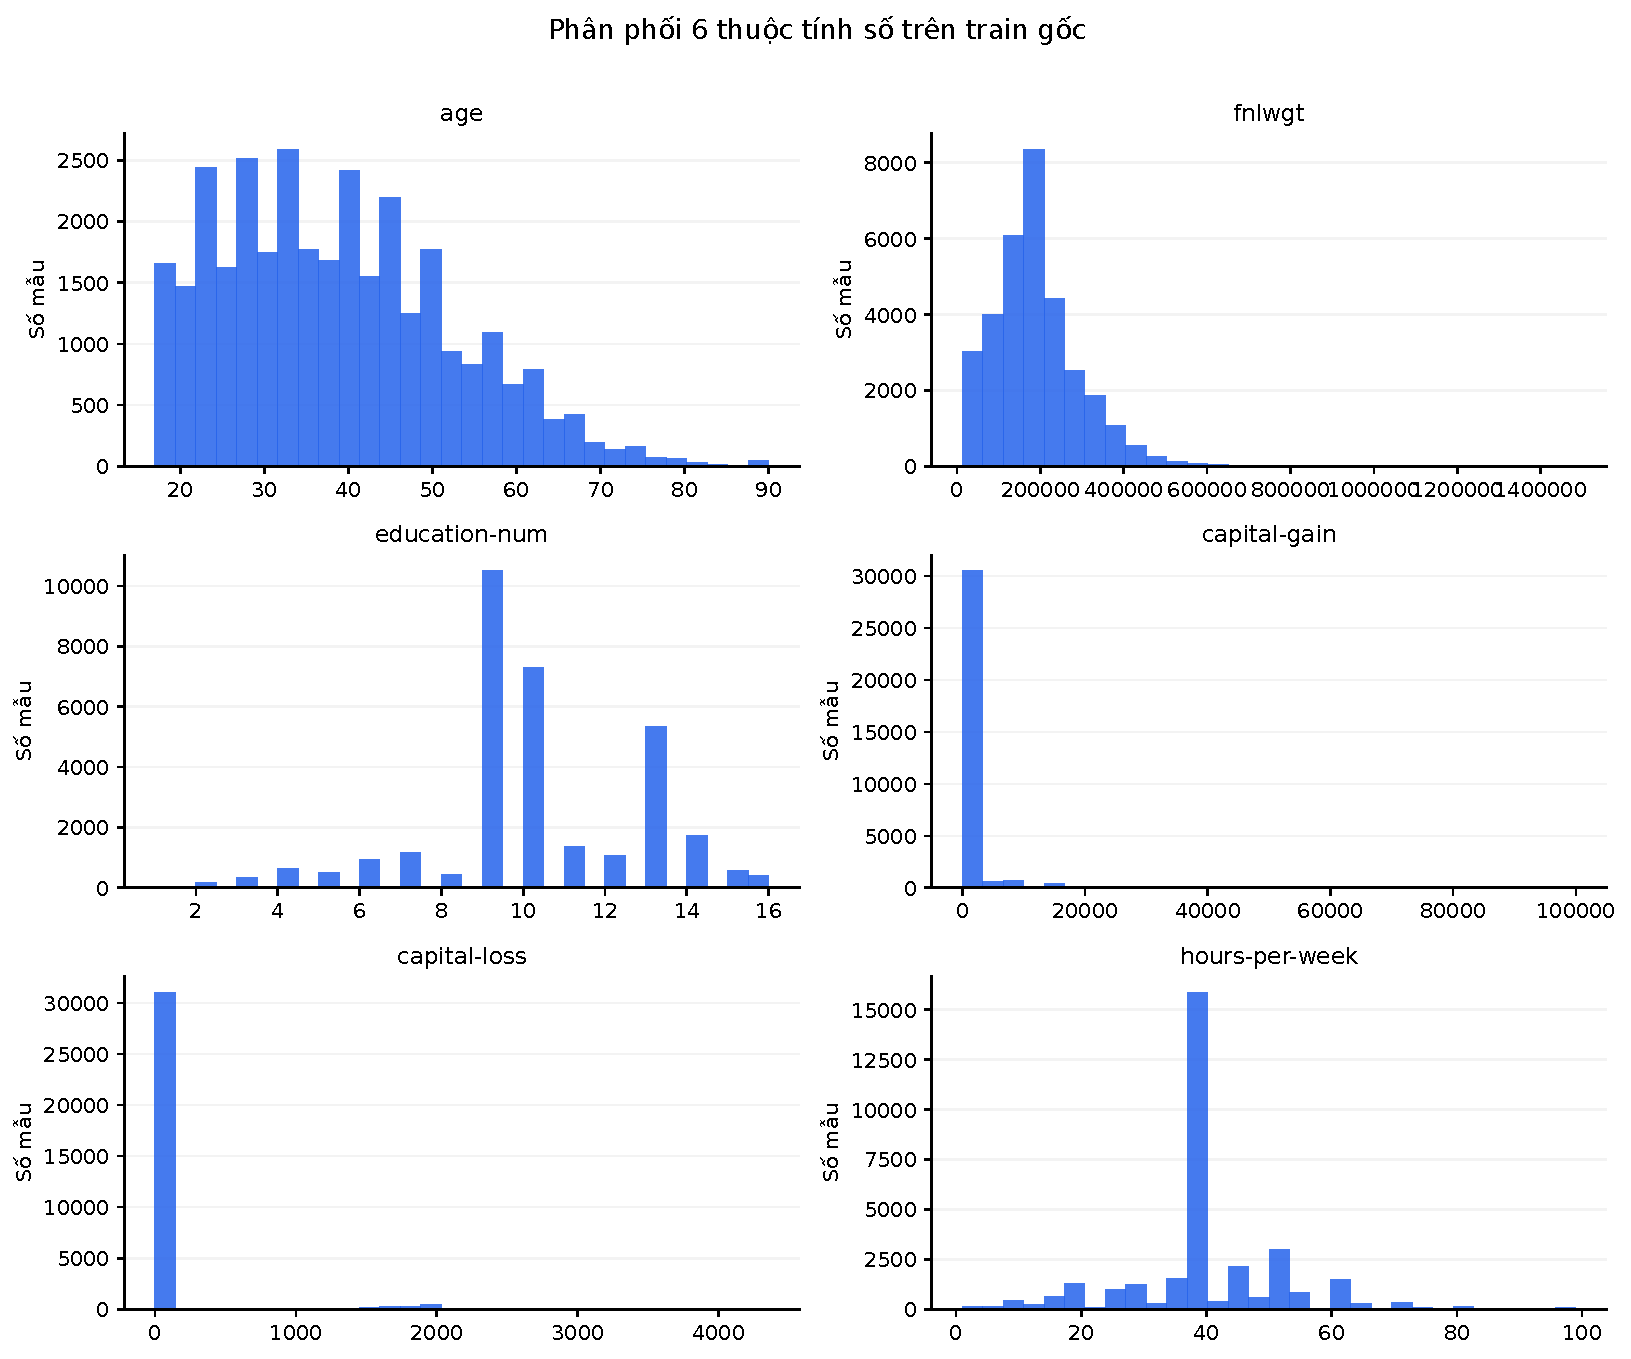
\includegraphics[width=.92\textwidth,height=.72\textheight,keepaspectratio]{Images/chapter_3/3_5/numeric_histograms.pdf}
\caption{Histogram của sáu thuộc tính số; không loại điểm cực trị}
\label{fig:numeric-histograms}
\end{figure}
